% Build from the repository root:
%   (cd docs && make images/daq_diagram.pdf)
%   (cd docs/slides && latexmk -pdfxe -shell-escape -outdir=../tex 2026_09_24_sequences.tex)
% TeX figures build in docs/images; measurement plots remain in
% build/analysis/adc/20260924_comparator_response/.
% Shared FRIDA Beamer style. Start each slide deck with % Shared FRIDA Beamer style. Start each slide deck with % Shared FRIDA Beamer style. Start each slide deck with \input{style.tex}.
\documentclass[aspectratio=169,compress]{beamer}
\usepackage[T1]{fontenc}
\usepackage{lmodern,graphicx,xcolor,amsmath,booktabs,array,tikz,listings,etoolbox}

% Decks are built from docs/slides; figures live beside docs and in docs/images.
\graphicspath{{../}{./}}

\definecolor{NordBody}{HTML}{4C566A}
\definecolor{NordBlue}{HTML}{5E81AC}
\definecolor{NordRed}{HTML}{BF616A}
\definecolor{NordGreen}{HTML}{A3BE8C}
\definecolor{NordOrange}{HTML}{D08770}
\definecolor{NordPurple}{HTML}{B48EAD}
\definecolor{NordPanel}{HTML}{ECEFF4}

\newcommand{\framesource}{}
\BeforeBeginEnvironment{frame}{\gdef\framesource{}}
\newcommand{\slidesource}[1]{\gdef\framesource{#1}}
\setbeamertemplate{footline}{%
  \hbox{%
    \begin{beamercolorbox}[wd=.12\paperwidth,ht=2.7ex,dp=1.2ex,leftskip=1em]{page number in head/foot}%
      \usebeamerfont{page number in head/foot}\insertframenumber\,/\,\inserttotalframenumber
    \end{beamercolorbox}%
    \begin{beamercolorbox}[wd=.88\paperwidth,ht=2.7ex,dp=1.2ex,right,rightskip=1em]{normal text}%
      \fontsize{5.5}{6.5}\selectfont\ifx\framesource\empty\else Sources:\enspace\framesource\fi
    \end{beamercolorbox}%
  }%
}
\beamertemplatenavigationsymbolsempty
\setbeameroption{hide notes}

% Opt in for decks with sections; shorter decks keep the full frame height.
\newcommand{\slideprogressnavigation}{%
  \useoutertheme[subsection=false]{miniframes}
  \setbeamercolor{section in head/foot}{fg=NordBlue,bg=white}
  \setbeamercolor{mini frame}{fg=NordBlue,bg=white}
  \setbeamercolor{lower separation line head}{bg=NordPanel}
  \setbeamerfont{section in head/foot}{size=\tiny}

  \newif\ifnavbeforecurrent
  \pretocmd\insertnavigation{\navbeforecurrenttrue}{}{}

  \newcommand{\fridanavigationdot}{%
    \begin{pgfpicture}{0pt}{0pt}{0.1cm}{0.1cm}
      \pgfpathcircle{\pgfpoint{0.05cm}{0.05cm}}{0.05cm}
      \ifnavbeforecurrent
        \pgfusepath{fill,stroke}
      \else
        \pgfusepath{stroke}
      \fi
    \end{pgfpicture}%
  }

  \defbeamertemplate*{mini frame}{frida progress}{%
    \begin{pgfpicture}{0pt}{0pt}{0.1cm}{0.1cm}
      \pgfpathcircle{\pgfpoint{0.05cm}{0.05cm}}{0.05cm}
      \pgfusepath{fill,stroke}
    \end{pgfpicture}%
    \global\navbeforecurrentfalse
  }
  \defbeamertemplate*{mini frame in current section}{frida progress}{\fridanavigationdot}
  \defbeamertemplate*{mini frame in current subsection}{frida progress}{\fridanavigationdot}
  \defbeamertemplate*{mini frame in other section}{frida progress}{\fridanavigationdot}
  \defbeamertemplate*{mini frame in other subsection}{frida progress}{\fridanavigationdot}
  \setbeamertemplate{mini frame}[frida progress]
  \setbeamertemplate{mini frame in current section}[frida progress]
  \setbeamertemplate{mini frame in current subsection}[frida progress]
  \setbeamertemplate{mini frame in other section}[frida progress]
  \setbeamertemplate{mini frame in other subsection}[frida progress]
}

\setbeamerfont{frametitle}{size=\large}
\setbeamerfont{framesubtitle}{size=\small}
\setbeamercolor{normal text}{fg=NordBody}
\setbeamercolor{title}{fg=NordBlue}
\setbeamercolor{frametitle}{fg=NordBlue}
\setbeamercolor{framesubtitle}{fg=NordBody}
\setbeamercolor{structure}{fg=NordBlue}
\setbeamercolor{itemize/enumerate body}{fg=NordBody}
\setbeamercolor{itemize/enumerate subbody}{fg=NordBody}
\setbeamercolor{itemize/enumerate subsubbody}{fg=NordBody}
\setbeamercolor{itemize item}{fg=NordBlue}
\setbeamercolor{itemize subitem}{fg=NordBlue}
\setbeamercolor{itemize subsubitem}{fg=NordBlue}
\setbeamercolor{enumerate item}{fg=NordBlue}
\setbeamercolor{enumerate subitem}{fg=NordBlue}
\setbeamercolor{enumerate subsubitem}{fg=NordBlue}
\setbeamercolor{block title}{fg=NordBlue,bg=NordPanel}
\setbeamercolor{block body}{fg=NordBody,bg=NordPanel!55}
\hypersetup{colorlinks=true,allcolors=NordBlue}

\lstset{%
  basicstyle=\ttfamily\tiny,
  keywordstyle=\color{NordBlue}\bfseries,
  commentstyle=\color{NordBody}\itshape,
  stringstyle=\color{NordOrange},
  showstringspaces=false,
  breaklines=true,
  frame=single,
  backgroundcolor=\color{NordPanel!55},
  rulecolor=\color{NordBody!50},
  xleftmargin=2pt,
  xrightmargin=2pt,
  aboveskip=4pt,
  belowskip=4pt,
}

\newcommand{\placeholder}[2]{%
  \begin{tikzpicture}
    \node[minimum width=#1,minimum height=#2,draw=NordBlue!60,rounded corners=2pt,fill=NordPanel,align=center,text=NordBody]
      {Placeholder\\[-1pt]\scriptsize image not yet available};
  \end{tikzpicture}%
}
\newcommand{\maybeimage}[2][]{%
  \IfFileExists{#2}{\includegraphics[#1]{#2}}{%
    \IfFileExists{../#2}{\includegraphics[#1]{#2}}{\placeholder{0.95\linewidth}{0.30\textheight}}%
  }%
}

\author{Kennedy Caisley}
\institute{University of Bonn}
.
\documentclass[aspectratio=169,compress]{beamer}
\usepackage[T1]{fontenc}
\usepackage{lmodern,graphicx,xcolor,amsmath,booktabs,array,tikz,listings,etoolbox}

% Decks are built from docs/slides; figures live beside docs and in docs/images.
\graphicspath{{../}{./}}

\definecolor{NordBody}{HTML}{4C566A}
\definecolor{NordBlue}{HTML}{5E81AC}
\definecolor{NordRed}{HTML}{BF616A}
\definecolor{NordGreen}{HTML}{A3BE8C}
\definecolor{NordOrange}{HTML}{D08770}
\definecolor{NordPurple}{HTML}{B48EAD}
\definecolor{NordPanel}{HTML}{ECEFF4}

\newcommand{\framesource}{}
\BeforeBeginEnvironment{frame}{\gdef\framesource{}}
\newcommand{\slidesource}[1]{\gdef\framesource{#1}}
\setbeamertemplate{footline}{%
  \hbox{%
    \begin{beamercolorbox}[wd=.12\paperwidth,ht=2.7ex,dp=1.2ex,leftskip=1em]{page number in head/foot}%
      \usebeamerfont{page number in head/foot}\insertframenumber\,/\,\inserttotalframenumber
    \end{beamercolorbox}%
    \begin{beamercolorbox}[wd=.88\paperwidth,ht=2.7ex,dp=1.2ex,right,rightskip=1em]{normal text}%
      \fontsize{5.5}{6.5}\selectfont\ifx\framesource\empty\else Sources:\enspace\framesource\fi
    \end{beamercolorbox}%
  }%
}
\beamertemplatenavigationsymbolsempty
\setbeameroption{hide notes}

% Opt in for decks with sections; shorter decks keep the full frame height.
\newcommand{\slideprogressnavigation}{%
  \useoutertheme[subsection=false]{miniframes}
  \setbeamercolor{section in head/foot}{fg=NordBlue,bg=white}
  \setbeamercolor{mini frame}{fg=NordBlue,bg=white}
  \setbeamercolor{lower separation line head}{bg=NordPanel}
  \setbeamerfont{section in head/foot}{size=\tiny}

  \newif\ifnavbeforecurrent
  \pretocmd\insertnavigation{\navbeforecurrenttrue}{}{}

  \newcommand{\fridanavigationdot}{%
    \begin{pgfpicture}{0pt}{0pt}{0.1cm}{0.1cm}
      \pgfpathcircle{\pgfpoint{0.05cm}{0.05cm}}{0.05cm}
      \ifnavbeforecurrent
        \pgfusepath{fill,stroke}
      \else
        \pgfusepath{stroke}
      \fi
    \end{pgfpicture}%
  }

  \defbeamertemplate*{mini frame}{frida progress}{%
    \begin{pgfpicture}{0pt}{0pt}{0.1cm}{0.1cm}
      \pgfpathcircle{\pgfpoint{0.05cm}{0.05cm}}{0.05cm}
      \pgfusepath{fill,stroke}
    \end{pgfpicture}%
    \global\navbeforecurrentfalse
  }
  \defbeamertemplate*{mini frame in current section}{frida progress}{\fridanavigationdot}
  \defbeamertemplate*{mini frame in current subsection}{frida progress}{\fridanavigationdot}
  \defbeamertemplate*{mini frame in other section}{frida progress}{\fridanavigationdot}
  \defbeamertemplate*{mini frame in other subsection}{frida progress}{\fridanavigationdot}
  \setbeamertemplate{mini frame}[frida progress]
  \setbeamertemplate{mini frame in current section}[frida progress]
  \setbeamertemplate{mini frame in current subsection}[frida progress]
  \setbeamertemplate{mini frame in other section}[frida progress]
  \setbeamertemplate{mini frame in other subsection}[frida progress]
}

\setbeamerfont{frametitle}{size=\large}
\setbeamerfont{framesubtitle}{size=\small}
\setbeamercolor{normal text}{fg=NordBody}
\setbeamercolor{title}{fg=NordBlue}
\setbeamercolor{frametitle}{fg=NordBlue}
\setbeamercolor{framesubtitle}{fg=NordBody}
\setbeamercolor{structure}{fg=NordBlue}
\setbeamercolor{itemize/enumerate body}{fg=NordBody}
\setbeamercolor{itemize/enumerate subbody}{fg=NordBody}
\setbeamercolor{itemize/enumerate subsubbody}{fg=NordBody}
\setbeamercolor{itemize item}{fg=NordBlue}
\setbeamercolor{itemize subitem}{fg=NordBlue}
\setbeamercolor{itemize subsubitem}{fg=NordBlue}
\setbeamercolor{enumerate item}{fg=NordBlue}
\setbeamercolor{enumerate subitem}{fg=NordBlue}
\setbeamercolor{enumerate subsubitem}{fg=NordBlue}
\setbeamercolor{block title}{fg=NordBlue,bg=NordPanel}
\setbeamercolor{block body}{fg=NordBody,bg=NordPanel!55}
\hypersetup{colorlinks=true,allcolors=NordBlue}

\lstset{%
  basicstyle=\ttfamily\tiny,
  keywordstyle=\color{NordBlue}\bfseries,
  commentstyle=\color{NordBody}\itshape,
  stringstyle=\color{NordOrange},
  showstringspaces=false,
  breaklines=true,
  frame=single,
  backgroundcolor=\color{NordPanel!55},
  rulecolor=\color{NordBody!50},
  xleftmargin=2pt,
  xrightmargin=2pt,
  aboveskip=4pt,
  belowskip=4pt,
}

\newcommand{\placeholder}[2]{%
  \begin{tikzpicture}
    \node[minimum width=#1,minimum height=#2,draw=NordBlue!60,rounded corners=2pt,fill=NordPanel,align=center,text=NordBody]
      {Placeholder\\[-1pt]\scriptsize image not yet available};
  \end{tikzpicture}%
}
\newcommand{\maybeimage}[2][]{%
  \IfFileExists{#2}{\includegraphics[#1]{#2}}{%
    \IfFileExists{../#2}{\includegraphics[#1]{#2}}{\placeholder{0.95\linewidth}{0.30\textheight}}%
  }%
}

\author{Kennedy Caisley}
\institute{University of Bonn}
.
\documentclass[aspectratio=169,compress]{beamer}
\usepackage[T1]{fontenc}
\usepackage{lmodern,graphicx,xcolor,amsmath,booktabs,array,tikz,listings,etoolbox}

% Decks are built from docs/slides; figures live beside docs and in docs/images.
\graphicspath{{../}{./}}

\definecolor{NordBody}{HTML}{4C566A}
\definecolor{NordBlue}{HTML}{5E81AC}
\definecolor{NordRed}{HTML}{BF616A}
\definecolor{NordGreen}{HTML}{A3BE8C}
\definecolor{NordOrange}{HTML}{D08770}
\definecolor{NordPurple}{HTML}{B48EAD}
\definecolor{NordPanel}{HTML}{ECEFF4}

\newcommand{\framesource}{}
\BeforeBeginEnvironment{frame}{\gdef\framesource{}}
\newcommand{\slidesource}[1]{\gdef\framesource{#1}}
\setbeamertemplate{footline}{%
  \hbox{%
    \begin{beamercolorbox}[wd=.12\paperwidth,ht=2.7ex,dp=1.2ex,leftskip=1em]{page number in head/foot}%
      \usebeamerfont{page number in head/foot}\insertframenumber\,/\,\inserttotalframenumber
    \end{beamercolorbox}%
    \begin{beamercolorbox}[wd=.88\paperwidth,ht=2.7ex,dp=1.2ex,right,rightskip=1em]{normal text}%
      \fontsize{5.5}{6.5}\selectfont\ifx\framesource\empty\else Sources:\enspace\framesource\fi
    \end{beamercolorbox}%
  }%
}
\beamertemplatenavigationsymbolsempty
\setbeameroption{hide notes}

% Opt in for decks with sections; shorter decks keep the full frame height.
\newcommand{\slideprogressnavigation}{%
  \useoutertheme[subsection=false]{miniframes}
  \setbeamercolor{section in head/foot}{fg=NordBlue,bg=white}
  \setbeamercolor{mini frame}{fg=NordBlue,bg=white}
  \setbeamercolor{lower separation line head}{bg=NordPanel}
  \setbeamerfont{section in head/foot}{size=\tiny}

  \newif\ifnavbeforecurrent
  \pretocmd\insertnavigation{\navbeforecurrenttrue}{}{}

  \newcommand{\fridanavigationdot}{%
    \begin{pgfpicture}{0pt}{0pt}{0.1cm}{0.1cm}
      \pgfpathcircle{\pgfpoint{0.05cm}{0.05cm}}{0.05cm}
      \ifnavbeforecurrent
        \pgfusepath{fill,stroke}
      \else
        \pgfusepath{stroke}
      \fi
    \end{pgfpicture}%
  }

  \defbeamertemplate*{mini frame}{frida progress}{%
    \begin{pgfpicture}{0pt}{0pt}{0.1cm}{0.1cm}
      \pgfpathcircle{\pgfpoint{0.05cm}{0.05cm}}{0.05cm}
      \pgfusepath{fill,stroke}
    \end{pgfpicture}%
    \global\navbeforecurrentfalse
  }
  \defbeamertemplate*{mini frame in current section}{frida progress}{\fridanavigationdot}
  \defbeamertemplate*{mini frame in current subsection}{frida progress}{\fridanavigationdot}
  \defbeamertemplate*{mini frame in other section}{frida progress}{\fridanavigationdot}
  \defbeamertemplate*{mini frame in other subsection}{frida progress}{\fridanavigationdot}
  \setbeamertemplate{mini frame}[frida progress]
  \setbeamertemplate{mini frame in current section}[frida progress]
  \setbeamertemplate{mini frame in current subsection}[frida progress]
  \setbeamertemplate{mini frame in other section}[frida progress]
  \setbeamertemplate{mini frame in other subsection}[frida progress]
}

\setbeamerfont{frametitle}{size=\large}
\setbeamerfont{framesubtitle}{size=\small}
\setbeamercolor{normal text}{fg=NordBody}
\setbeamercolor{title}{fg=NordBlue}
\setbeamercolor{frametitle}{fg=NordBlue}
\setbeamercolor{framesubtitle}{fg=NordBody}
\setbeamercolor{structure}{fg=NordBlue}
\setbeamercolor{itemize/enumerate body}{fg=NordBody}
\setbeamercolor{itemize/enumerate subbody}{fg=NordBody}
\setbeamercolor{itemize/enumerate subsubbody}{fg=NordBody}
\setbeamercolor{itemize item}{fg=NordBlue}
\setbeamercolor{itemize subitem}{fg=NordBlue}
\setbeamercolor{itemize subsubitem}{fg=NordBlue}
\setbeamercolor{enumerate item}{fg=NordBlue}
\setbeamercolor{enumerate subitem}{fg=NordBlue}
\setbeamercolor{enumerate subsubitem}{fg=NordBlue}
\setbeamercolor{block title}{fg=NordBlue,bg=NordPanel}
\setbeamercolor{block body}{fg=NordBody,bg=NordPanel!55}
\hypersetup{colorlinks=true,allcolors=NordBlue}

\lstset{%
  basicstyle=\ttfamily\tiny,
  keywordstyle=\color{NordBlue}\bfseries,
  commentstyle=\color{NordBody}\itshape,
  stringstyle=\color{NordOrange},
  showstringspaces=false,
  breaklines=true,
  frame=single,
  backgroundcolor=\color{NordPanel!55},
  rulecolor=\color{NordBody!50},
  xleftmargin=2pt,
  xrightmargin=2pt,
  aboveskip=4pt,
  belowskip=4pt,
}

\newcommand{\placeholder}[2]{%
  \begin{tikzpicture}
    \node[minimum width=#1,minimum height=#2,draw=NordBlue!60,rounded corners=2pt,fill=NordPanel,align=center,text=NordBody]
      {Placeholder\\[-1pt]\scriptsize image not yet available};
  \end{tikzpicture}%
}
\newcommand{\maybeimage}[2][]{%
  \IfFileExists{#2}{\includegraphics[#1]{#2}}{%
    \IfFileExists{../#2}{\includegraphics[#1]{#2}}{\placeholder{0.95\linewidth}{0.30\textheight}}%
  }%
}

\author{Kennedy Caisley}
\institute{University of Bonn}


\usetikzlibrary{calc}

\newcommand{\systemdiagram}{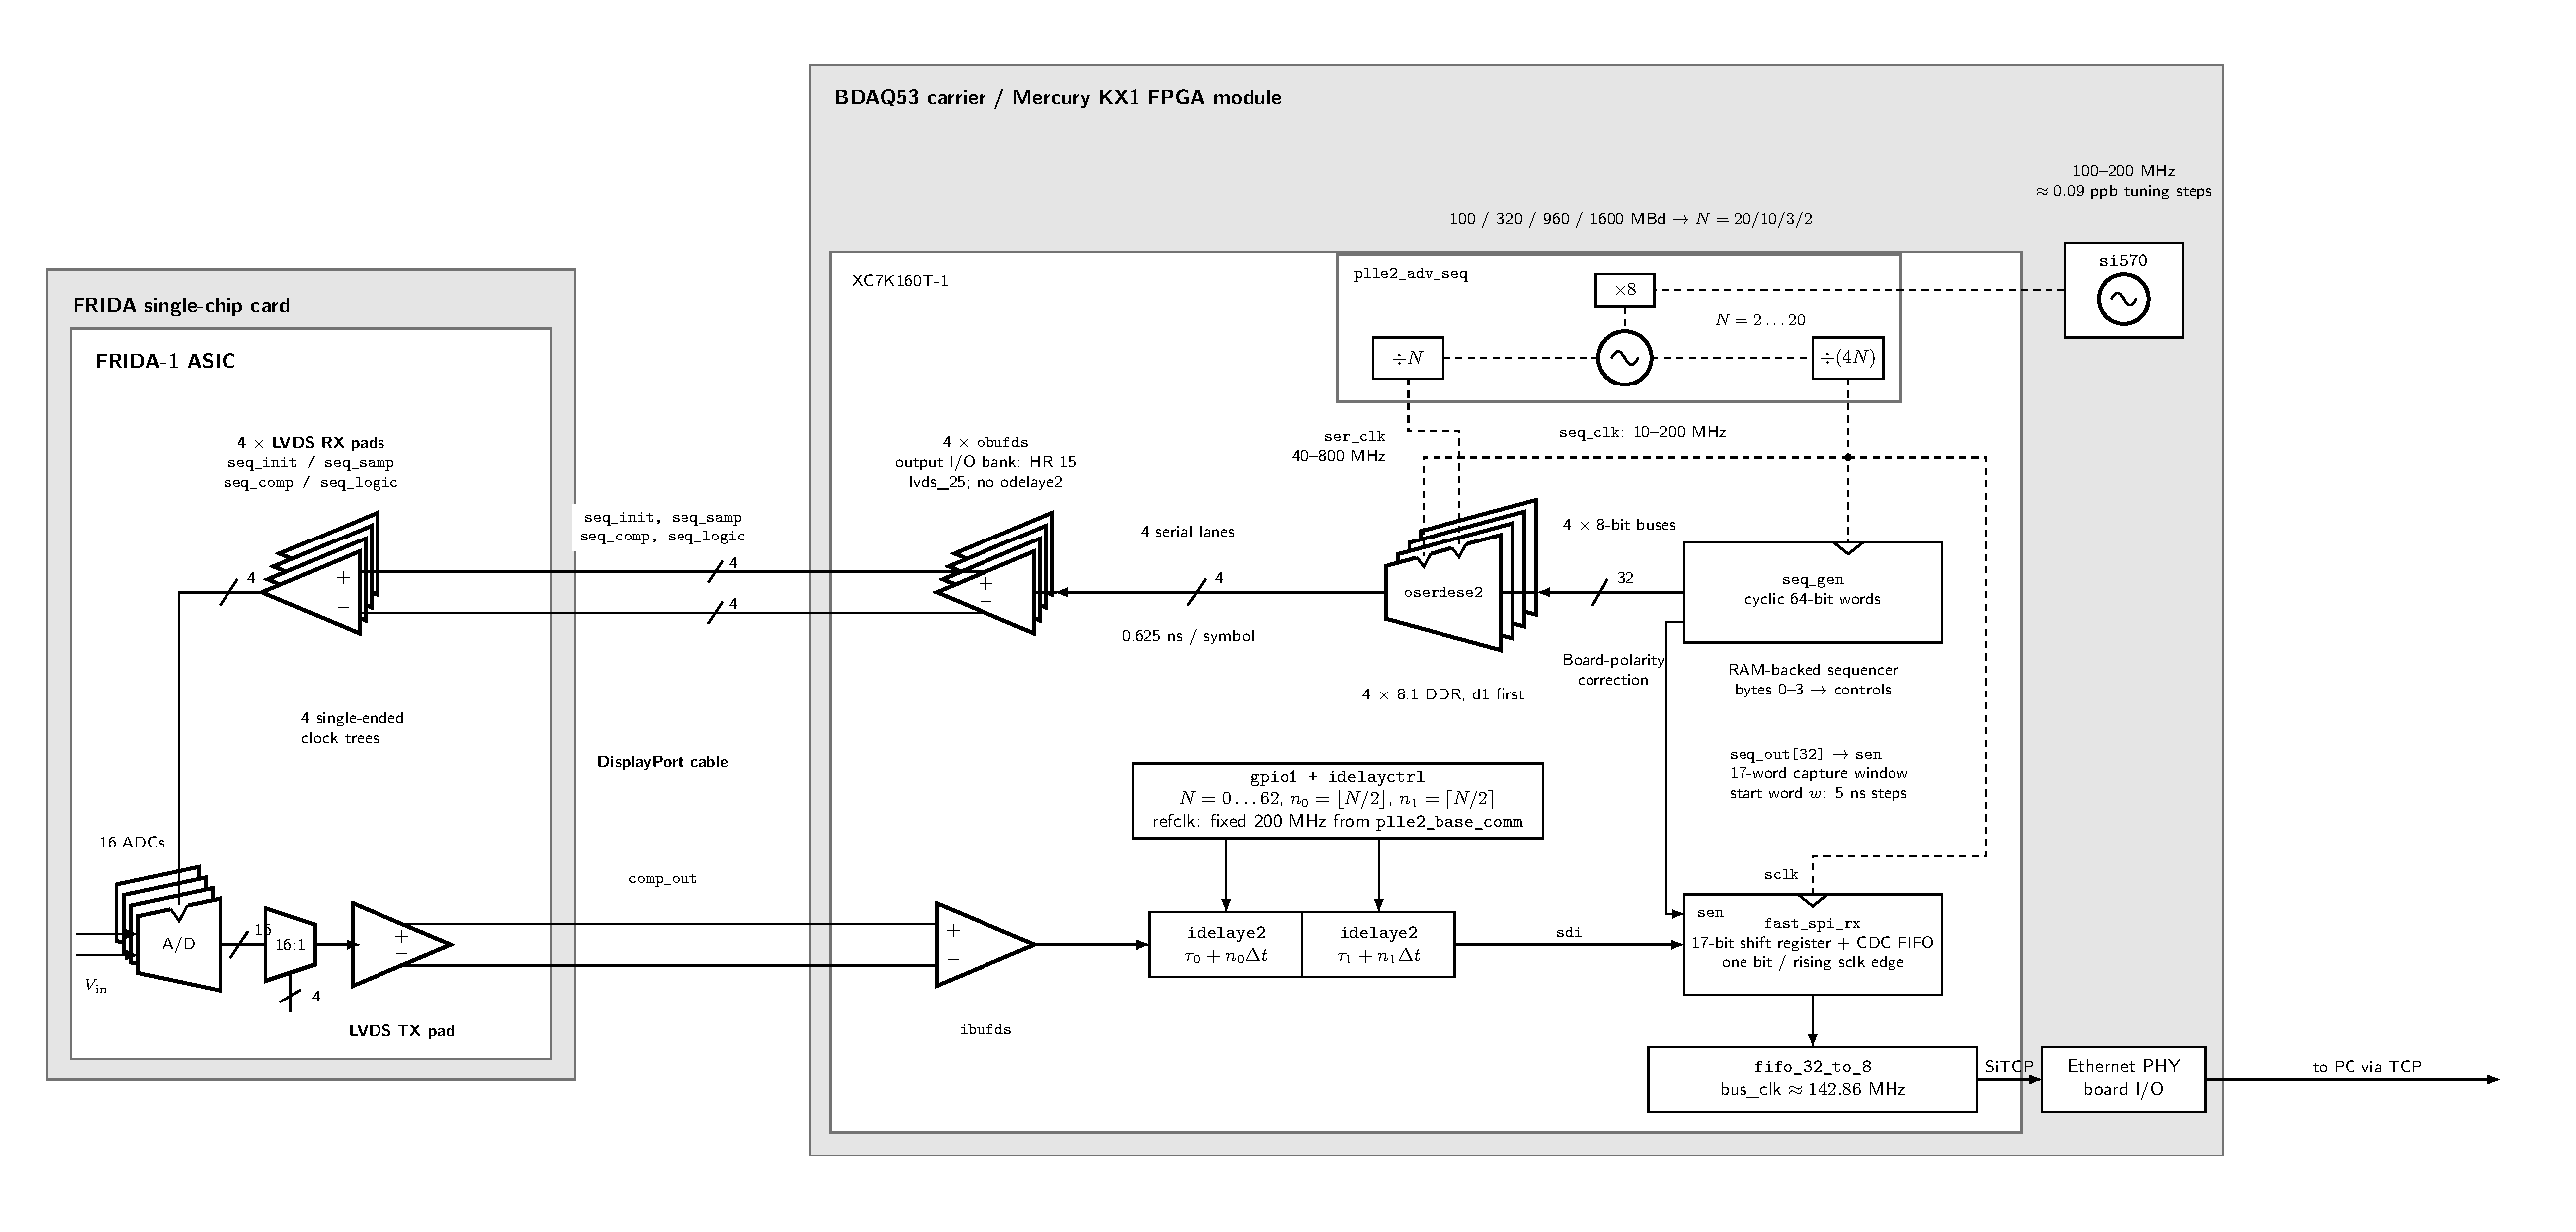
\includegraphics[width=0.98\paperwidth,height=0.80\paperheight,keepaspectratio]{../images/daq_diagram.pdf}}
\newcommand{\qdelay}[1]{\textcolor{NordRed}{$t_{d,\mathrm{#1}}$=?}}
\newcommand{\vdelay}[2]{\textcolor{NordBlue}{$t_{d,\mathrm{#1}}=#2$}}
\newcommand{\progressframe}[6]{%
  \begin{frame}{#1}
    \centering
    \makebox[\linewidth][c]{\begin{tikzpicture}
      \node[inner sep=0pt] (diagram) {\systemdiagram};
      \begin{scope}[
        shift={(diagram.south west)},
        x={($(diagram.south east)-(diagram.south west)$)},
        y={($(diagram.north west)-(diagram.south west)$)},
        timing/.style={inner sep=0pt,align=center,font=\fontsize{4}{4.5}\selectfont}
      ]
        \node[timing] at (0.45,0.40) {#2};
        \node[timing] at (0.17,0.37) {#3};
        \node[timing] at (0.15,0.32) {#4};
        \node[timing] at (0.28,0.15) {#5};
        \node[timing] at (0.54,0.17) {#6};
      \end{scope}
    \end{tikzpicture}}
    \note{The image uses exactly the same scale as the opening diagram. Small red timing unknowns on the diagram become blue values as each segment is characterized.}
  \end{frame}%
}

\title{Timing the FRIDA ADC capture loop}
\date{24 September 2026}

\begin{document}

\begin{frame}
  \titlepage
\end{frame}

\begin{frame}{FRIDA DAQ path}
  \centering
  \makebox[\linewidth][c]{\systemdiagram}
  \note{Source: docs/images/daq_diagram.tex. Later slides overlay the timing measurements on this diagram one segment at a time.}
\end{frame}

\begin{frame}{Four ADC control rows}
  \centering
  \IfFileExists{../images/sequences/comp11110000_logic00001111.pdf}{%
    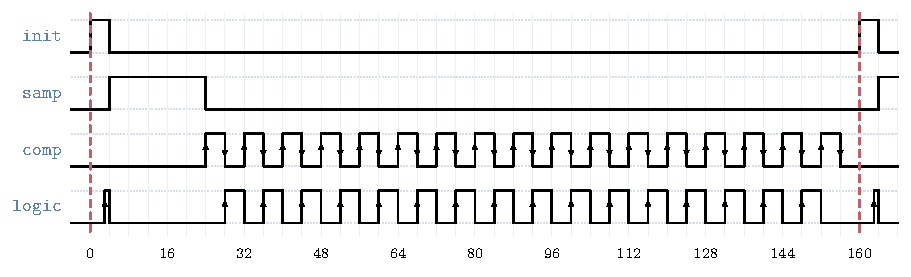
\includegraphics[width=0.94\linewidth,height=0.69\textheight,keepaspectratio]{../images/sequences/comp11110000_logic00001111.pdf}%
  }{%
    \begin{tabular}{@{}ll@{}}
      INIT & four high symbols at the conversion start \\
      SAMP & twenty high symbols after INIT \\
      COMP & \texttt{11110000}, repeated for 17 decisions \\
      LOGIC & \texttt{00001111} at each decision \\
    \end{tabular}%
  }
  \par\smallskip
  {\small 160 symbols\qquad1.6 GBd\qquad100 ns repeat\qquad17 COMP rises\qquad5 ns spacing}
  \note{Sources: docs/images/sequences/comp11110000_logic00001111.tex, flow/adc/sequences.py, docs/usage.md Hardware ADC acquisition. The drawing includes the first 5 ns of the next conversion to show the 100 ns boundary.}
\end{frame}

\progressframe{Timing terms}
  {\qdelay{TX}\\\textcolor{NordRed}{$\sigma_{t,\mathrm{TX}}$=?}}
  {\qdelay{ASIC,RX}}
  {\qdelay{XC}\\\qdelay{SR}}
  {\qdelay{ASIC,TX}}
  {\qdelay{FPGA,RX}}

\begin{frame}{FPGA TX timing}
  \begin{columns}[T,onlytextwidth]
    \begin{column}{0.53\textwidth}
      \large
      \begin{align*}
        t_{\rm OSERDES} &= 0.192\text{--}0.415\ \mathrm{ns},\\
        t_{\rm OBUFDS} &= 0.818\text{--}1.589\ \mathrm{ns},\\
        t_{\rm TX,pad} &= 1.010\text{--}2.004\ \mathrm{ns}.
      \end{align*}
    \end{column}
    \begin{column}{0.44\textwidth}
      \large
      $\sigma_{t,\mathrm{COMP},0}=18.7\ \mathrm{ps}$ RMS\par\medskip
      256 scope captures
    \end{column}
  \end{columns}
  \note{The output path report is OSERDESE2 CLK to CLK_COMP_P at zero external load. The 18.7 ps figure is scope trigger-referenced first-edge spread across 256 captures. A separate FPGA COMP output-eye run is archived and shown next.}
\end{frame}

\begin{frame}{FPGA sequencer and serializer output}
  \centering
  \includegraphics[width=0.98\linewidth,height=0.94\textheight,keepaspectratio]{../../build/analysis/adc/20260924_comparator_response/msmt_fpga_serdes_output_words_grid.pdf}
  \note{32 scope captures per case, seven eight-symbol words at 320, 960, and 1600 MBd. The small traces above the columns show the ideal programmed words.}
\end{frame}

\begin{frame}{FPGA serializer symbol eye}
  \centering
  \includegraphics[width=0.98\linewidth,height=0.90\textheight,keepaspectratio]{../../build/analysis/adc/20260924_comparator_response/msmt_fpga_serdes_symbol_eye.pdf}
  \note{A single 256-bit pattern covers all 254 nonconstant cyclic eight-bit contexts. Each measured symbol is folded into one unit interval; the plots show all contexts at 320, 960, and 1600 MBd.}
\end{frame}

\begin{frame}{ADC03 scope: full sequence at 320 MBd}
  \centering
  \includegraphics[width=0.98\linewidth,height=0.82\textheight,keepaspectratio]{../../build/analysis/adc/20260924_comparator_response/msmt_adc03_full_sequence_320mbd.pdf}
  \note{ADC03 no-control scan, fixed plus 50 mV differential input, CH1 INIT scope trigger. The window includes all 17 COMP decisions and the next INIT boundary.}
\end{frame}

\begin{frame}{ADC03 scope: full sequence at 960 MBd}
  \centering
  \includegraphics[width=0.98\linewidth,height=0.82\textheight,keepaspectratio]{../../build/analysis/adc/20260924_comparator_response/msmt_adc03_full_sequence_960mbd.pdf}
  \note{ADC03 no-control scan, fixed plus 50 mV differential input, CH1 INIT scope trigger. The window includes all 17 COMP decisions and the next INIT boundary.}
\end{frame}

\begin{frame}{ADC03 scope: full sequence at 1600 MBd}
  \centering
  \includegraphics[width=0.98\linewidth,height=0.82\textheight,keepaspectratio]{../../build/analysis/adc/20260924_comparator_response/msmt_adc03_full_sequence_1600mbd.pdf}
  \note{ADC03 no-control scan, fixed plus 50 mV differential input, CH1 INIT scope trigger. The window includes all 17 COMP decisions and the next INIT boundary.}
\end{frame}

\progressframe{FPGA TX delay}
  {\vdelay{TX}{1.01\text{--}2.00\,\mathrm{ns}}\\\textcolor{NordRed}{$\sigma_{t,\mathrm{TX}}$=?}}
  {\qdelay{ASIC,RX}}
  {\qdelay{XC}\\\qdelay{SR}}
  {\qdelay{ASIC,TX}}
  {\qdelay{FPGA,RX}}

\begin{frame}{FRIDA clock-input delay (ns)}
  \centering
  \large
  \begin{tabular}{@{}lrrr@{}}
    \toprule
    Segment & FF & TT & SS \\
    \midrule
    COMP pad $\to$ RX output & 0.207 & 0.246 & 0.304 \\
    COMP pad $\to$ latch clock & 0.359 & \textbf{0.432} & 0.532 \\
    \bottomrule
  \end{tabular}
  \par\medskip
  {\normalsize TT clock tree and gate: 0.185 ns}
  \note{The numerical table is copied from the pruned full-chip Spectre bench. The 0.432 ns is measured from differential pad zero crossing to internal comp_latch.CLK half-supply crossing.}
\end{frame}

\progressframe{FRIDA clock-input delay}
  {\vdelay{TX}{1.01\text{--}2.00\,\mathrm{ns}}\\\textcolor{NordRed}{$\sigma_{t,\mathrm{TX}}$=?}}
  {\vdelay{ASIC,RX}{0.359\text{--}0.532\,\mathrm{ns}}}
  {\qdelay{XC}\\\qdelay{SR}}
  {\qdelay{ASIC,TX}}
  {\qdelay{FPGA,RX}}

\begin{frame}{PEX comparator waveforms: 10 MSPS}
  \centering
  \includegraphics[width=0.99\linewidth,height=0.78\textheight,keepaspectratio]{../../build/analysis/adc/20260924_comparator_response/sim_10msps_edge_eye_timing.pdf}
\end{frame}

\begin{frame}{PEX comparator decision eye: 10 MSPS}
  \centering
  \includegraphics[width=0.99\linewidth,height=0.78\textheight,keepaspectratio]{../../build/analysis/adc/20260924_comparator_response/sim_10msps_edge_eye_decision_eye.pdf}
\end{frame}

\begin{frame}{PEX comparator response: 10 MSPS}
  \centering
  \includegraphics[width=0.98\linewidth,height=0.73\textheight,keepaspectratio]{../../build/analysis/adc/20260924_comparator_response/sim_10msps_response.pdf}
  \par\smallskip
  {\small 100 conversions\qquad XC valid: 1677/1700\qquad SR transitions: 1129\qquad SR held: 443}
  \note{The 160-symbol PEX case runs at 1600 MBd and 10 MSPS. XC validity requires opposite rails around 50 percent VDD before COMP reset. Twenty-three XC decisions remain unresolved. The archived 168-symbol case runs at 9.52 MSPS and is not a 100 ns candidate.}
\end{frame}

\progressframe{XC and SR response}
  {\vdelay{TX}{1.01\text{--}2.00\,\mathrm{ns}}\\\textcolor{NordRed}{$\sigma_{t,\mathrm{TX}}$=?}}
  {\vdelay{ASIC,RX}{0.359\text{--}0.532\,\mathrm{ns}}}
  {\vdelay{XC}{0.86\text{--}2.03\,\mathrm{ns}}\\\vdelay{SR}{1.43\text{--}2.56\,\mathrm{ns}}}
  {\qdelay{ASIC,TX}}
  {\qdelay{FPGA,RX}}

\begin{frame}{FRIDA output delay (ns)}
  \centering
  \large
  \begin{tabular}{@{}lrrr@{}}
    \toprule
    SR latch $\to$ COMP\_OUT pad & FF & TT & SS \\
    \midrule
    Rising output & 0.476 & \textbf{0.560} & 0.660 \\
    Falling output & 0.501 & \textbf{0.586} & 0.689 \\
    \bottomrule
  \end{tabular}
  \par\medskip
  {\normalsize TT pad: 0.367 / 0.389 ns\qquad100 $\Omega$ differential\qquad1 pF / pad}
  \note{The path starts at comp_sr.LATCH_P and ends at the COMP_OUT differential pad zero crossing. Edge direction changes the delay.}
\end{frame}

\begin{frame}{Scope COMP and COMP\_OUT: 2 MSPS}
  \centering
  \includegraphics[width=0.98\linewidth,height=0.78\textheight,keepaspectratio]{../../build/analysis/adc/20260924_comparator_response/msmt_adc01_2msps_comp_timing.pdf}
  \note{Source: all 256 raw scope captures from build/test_fastrx/20260923_182335/comp_out_edge_eye, aligned to each capture's first COMP rising edge. The internal XC nodes are unavailable at the scope.}
\end{frame}

\begin{frame}{Scope COMP and COMP\_OUT decision eye: 2 MSPS}
  \centering
  \includegraphics[width=0.98\linewidth,height=0.78\textheight,keepaspectratio]{../../build/analysis/adc/20260924_comparator_response/msmt_adc01_2msps_comp_decision_eye.pdf}
  \note{Source: all 256 saved scope captures. All 17 decision windows from every capture are aligned to their COMP rising edge; 4352 windows are overlaid in the same format as the PEX decision eye.}
\end{frame}

\begin{frame}{Scope COMP\_OUT midpoint edge: 2 MSPS}
  \centering
  \includegraphics[width=0.98\linewidth,height=0.78\textheight,keepaspectratio]{../../build/analysis/adc/20260924_comparator_response/msmt_adc01_2msps_comp_response_histogram.pdf}
  \note{Per-decision normalized horizontal histograms of first COMP_OUT midpoint crossings after the scope COMP rise. Each bar's width is the fraction of changing captures in its time bin.}
\end{frame}

\progressframe{FRIDA output delay}
  {\vdelay{TX}{1.01\text{--}2.00\,\mathrm{ns}}\\\textcolor{NordRed}{$\sigma_{t,\mathrm{TX}}$=?}}
  {\vdelay{ASIC,RX}{0.359\text{--}0.532\,\mathrm{ns}}}
  {\vdelay{XC}{0.86\text{--}2.03\,\mathrm{ns}}\\\vdelay{SR}{1.43\text{--}2.56\,\mathrm{ns}}}
  {\vdelay{ASIC,TX}{0.476\text{--}0.689\,\mathrm{ns}}}
  {\qdelay{FPGA,RX}}

\begin{frame}{FPGA RX and capture clock}
  \begin{columns}[T,onlytextwidth]
    \begin{column}{0.52\textwidth}
      \large
      \begin{align*}
        t_{\rm pad\to D}(N{=}0) &= 3.309\text{--}7.271\ \mathrm{ns},\\
        \Delta t_{\rm tap} &= 78.125\ \mathrm{ps},\\
        0\leq N &\leq 62.
      \end{align*}
    \end{column}
    \begin{column}{0.45\textwidth}
      \large
      \begin{align*}
        t_{\rm capture\ clock} &= 4.222\text{--}8.706\ \mathrm{ns}.
      \end{align*}
    \end{column}
  \end{columns}
  \note{The 3.309 ns fast and 7.271 ns slow input-path values are from different PVT corners. Capture clock insertion must be paired with the corresponding launch corner, not subtracted from an arbitrary opposite-corner data path. The nominal total tap span is 4.84375 ns.}
\end{frame}

\begin{frame}{Measured FastRX capture settings}
  \centering
  \small
  \begin{tabular}{@{}lrrr@{}}
    \toprule
    Sequence period & Baud (MBd) & Combined taps $N$ & SEN word $w$ \\
    \midrule
    160 symbols & 320 & 16 & 5 \\
    160 symbols & 960 & 40 & 7 \\
    160 symbols & 1600 & 12 & 8 \\
    \midrule
    256 symbols & 320 & 31 & 6 \\
    256 symbols & 960 & 12 & 7 \\
    256 symbols & 1600 & 36 & 9 \\
    \bottomrule
  \end{tabular}
  \par\medskip
  {\normalsize 96 files $\times$ 10,000 conversions\qquad1632 / 1632 scope--FastRX decisions agree}
  \note{The 160-symbol rows correspond to 2, 6 and 10 MSPS. The 256-symbol rows correspond to 1.25, 3.75 and 6.25 MSPS at the same baud rates. Only one scope conversion per file was checked against FastRX.}
\end{frame}

\progressframe{Measured path terms}
  {\vdelay{TX}{1.01\text{--}2.00\,\mathrm{ns}}\\\textcolor{NordRed}{$\sigma_{t,\mathrm{TX}}$=?}}
  {\vdelay{ASIC,RX}{0.359\text{--}0.532\,\mathrm{ns}}}
  {\vdelay{XC}{0.86\text{--}2.03\,\mathrm{ns}}\\\vdelay{SR}{1.43\text{--}2.56\,\mathrm{ns}}}
  {\vdelay{ASIC,TX}{0.476\text{--}0.689\,\mathrm{ns}}}
  {\vdelay{FPGA,RX}{3.309\text{--}7.271\,\mathrm{ns}}\\\textcolor{NordBlue}{$+N\,78.125\,\mathrm{ps}$}}

\begin{frame}{Capture timing variables}
  \normalsize
  \begin{align*}
    T_s &= 1/B,\qquad T_w = 8/B,\qquad k_j=k_0+8j,\\[4pt]
    F_c &= t_{{\rm FPGA,TX},c}+t_{{\rm FPGA,RX0},c}
             -t_{{\rm capture\ clock},c},\\[4pt]
    F^- &= \min_c F_c,\qquad F^+ = \max_c F_c.
  \end{align*}
  \begin{align*}
    P &= \text{sequencer pipeline (words)},\\
    R^- &\leq t_{\rm COMP\ pad\to COMP\_OUT\ FPGA\ pin} \leq R^+.
  \end{align*}
  \note{Source: flow/scans/fastrx.py calculate_fastrx_capture_settings. The pipeline is an input parameter because it has not been established as a universal constant here. R cannot be filled directly from the raw scope measurement without probe, board and threshold alignment.}
\end{frame}

\begin{frame}{FastRX sample window}
  \large
  \begin{align*}
    t_{\rm latest}(j,N)
      &= k_j T_s+P T_w+R^+ + F^+ + N\Delta t,\\[5pt]
    t_{\rm next,earliest}(j,N)
      &= (k_j+8)T_s+P T_w+R^- + F^- + N\Delta t,\\[5pt]
    t_{\rm sample}(j,w) &= wT_w+jT_w.
  \end{align*}
  \normalsize
  \begin{align*}
    t_{\rm latest}+G_{\rm setup} &\leq t_{\rm sample},\\
    t_{\rm sample}+G_{\rm hold} &\leq t_{\rm next,earliest},\qquad j=0,\ldots,16.
  \end{align*}
  \note{The equal 8-symbol COMP spacing makes the j terms cancel for a complete 17-bit conversion. This is why the first comparator edge and the baud determine the word placement, provided the sequence is not rotated.}
\end{frame}

\begin{frame}{IDELAY taps and RX\_SEN word}
  \small
  \begin{align*}
    N_{\min}(w) &= \max\!\left(0,\left\lceil
      \frac{wT_w+G_{\rm hold}-k_0T_s-(P+1)T_w-R^- -F^-}{\Delta t}
      \right\rceil\right),\\[7pt]
    N_{\max}(w) &= \min\!\left(62,\left\lfloor
      \frac{wT_w-k_0T_s-PT_w-R^+ -F^+ -G_{\rm setup}}{\Delta t}
      \right\rfloor\right).
  \end{align*}
  \normalsize
  \begin{align*}
    N_{\min}(w)&\leq N\leq N_{\max}(w),\qquad 0\leq w<L/8,\\
    n_0&=\lfloor N/2\rfloor,\qquad n_1=\lceil N/2\rceil,\\
    \mathrm{RX\_SEN}&=1\quad\text{for 17 words from }w.
  \end{align*}
  \note{Source: flow/scans/fastrx.py calculate_fastrx_capture_settings and design/fpga/daq_top.v tap split. The implementation enumerates legal w and N to maximize the smaller margin; the inequalities shown are the equivalent interval form. The existing hardware profiles are still used until all R and F bounds, guards and pipeline are validated.}
\end{frame}

\end{document}
